% TODO introduire l'application, les fonctionnalités et les types d'user brièvement

\chapter{Analyse des besoins}
% Partie dans laquelle on explique les features / requirements attendues
% On y trouve sans doute :

\epigraph{<< Les choses paraissent simples jusqu'à ce qu'on commence à les analyser >>}{Audrey Niffenegger}

La phase d'analyse est dans la vie d'un projet l'une des phases les plus critiques car celle-ci formalise les besoins des clients sous tous ses aspects afin que toutes les parties (dont les développeurs) puissent se mettre d'accord. Pour pallier les nombreuses difficultés inhérentes au contexte, plusieurs méthodes reconnues existent (notamment \Gls{QQOQCCP} et UML). \\

La principale fonctionnalité attendue de l'application web est la recherche de fiches sur base d'une combinaison de critères divers et variés (dont notamment des mots-clés) pourrait sembler à première vue simple mais il n'en est rien. En effet, la question sous-jacente est le problème du référencement de ressources informatiques. Contrairement à d'autres domaines (par exemple la littérature), il n'existe pas de consensus sur au moins une manière d'organiser les informations d'une ressource informatique.

\section{Analyse fonctionnelle}

\subsection*{Séparation des tâches}

Comme expliqué par les Echos\cite{SOD}, la séparation des tâches est "un concept qui requière différents acteurs possédant des rôles et responsabilités différents pour la réalisation d’un ensemble de tâches dont l’exécution par un unique acteur pourrait potentiellement conduire à des fraudes ou des erreurs". \\


En effet, ce catalogue qui repose sur la collaboration d'acteurs variés nécessite un certain nombre de garde-fous afin de maintenir un outil qui dispose de ressources aussi bien de manière qualitative que quantitative. Notre analyse nous a permis d'isoler 4 types d'utilisateurs qui disposent de privilèges de manière incrémentale (en plus de disposer de leurs privilèges propres, chacun hérite aussi de ceux du précédent de la présente liste) :

\begin{itemize}
    \item Visiteur : Il s'agit d'un utilisateur non inscrit à notre plate-forme. Il ne peut rechercher et consulter que les fiches de ressources validés par un administrateur.
    \item Utilisateur : Il s'agit d'un utilisateur  inscrit à notre plate-forme. Celui-ci peut proposer des nouvelles ressources ainsi que de maintenir les fiches dont il est le créateur.
    \item Administrateur : Celui-ci crée/modifie des ressources de toute nature (fiches proposées par les utilisateurs, mots clés et catégories de mots clé), en plus de classifier les fiches.
    \item Super Administrateur : Celui-ci dispose du droit de supprimer de manière définitive les différentes ressources de notre plate-forme.
\end{itemize}

\subsection*{Fonctionnalités}

\subsubsection*{Tout visiteur peut : }

\begin{itemize}
    \item Se connecter à l'application via une adresse mail et un mot de passe
    \item S'inscrire à l'application
    \item Rechercher des fiches dans l'application. La recherche se porte sur une combinaison libre des critères suivants : 
    \begin{itemize}
        \item Rechercher dans le titre des fiches
        \item Rechercher dans les mots clés des fiches ( cf TODO : Ce point sera expliqué en détail au point x.z.y )
        \item Filtrer les fiches par leurs identifiants
        \item Filtrer les fiches par leurs créateurs
        \item Filtrer les fiches par leurs états
        \item Filtrer les fiches sur base d'un certain seuil sur le résultat moyen accordé par les utilisateurs
    \end{itemize}
    Il est également possible d'y associer les fonctionnalités suivantes :
    \begin{itemize}
        \item Ordonner les fiches avec une libre combinaison des paramètres suivants (en précisant pour chacun l'ordre du tri : ascendant / descendant) :
        \begin{itemize}
            \item le résultat moyen des votants pour une fiche
            \item le nombre de votants pour une fiche
            \item la date de la dernière modification de la fiche
            \item le titre de la fiche
            \item l'état de la fiche
            \item l'identifiant de la fiche
        \end{itemize}
        \item Choisir quelles propriétés des fiches inclure dans le résultat
    \end{itemize}
    \item Consulter une fiche
    \item Consulter les mots clés et catégories de mots clés existants ( avec si demandé, des statistiques d'utilisation de ceux ci )
    \item Télécharger la source d'une fiche 
\end{itemize}

\subsubsection*{Tout utilisateur peut : }
\begin{itemize}
    \item Consulter / Modifier ses informations personnelles
    \item Mettre en ligne une fiche (avec éventuellement un fichier )
    \item Modifier les informations d'une fiche l'appartenant
    \item Changer l'état d'une fiche l'appartenant ( des restrictions existent pour éviter des dérives )
    \item Proposer un nouveau ou plusieurs mot(s) clé(s)
    \item Évaluer une fiche 
    \item \Gls{crud} des recherches favorites
\end{itemize}

\subsubsection*{Tout administrateur peut : }
\begin{itemize}
    \item Exporter des fiches au format JSON
    \item Mettre en ligne plusieurs fiches (avec éventuellement un état spécifique pour chacune)
    \item Proposer un nouveau ou plusieurs mot(s) clé(s) (avec éventuellement un état spécifique pour chacun)
    \item Modifier un mot clé
    \item Modifier une catégorie de mots clés
    \item Changer l'état d'un ou plusieurs mot(s) clé(s)
    \item Modifier les informations d'une fiche
    \item Changer l'état d'une fiche ( aucune restriction)
    \item Créer ou trouver des catégories de mots clés
    \item Lister tous les utilisateurs de l'application ( sans distinction )
\end{itemize}

\subsubsection*{Tout super administrateur peut : }
\begin{itemize}
    \item Supprimer des fiches / mot(s) clé(s) / catégories de mots clés
    \item Modifier le type d'un utilisateur
\end{itemize}
\pagebreak
\subsection*{État d'une fiche}

Au cours de notre analyse des processus de partage/modération de ressources informatiques, nous avons été confrontés à de nombreuses lacunes dans des systèmes similaires dont notamment :
\begin{itemize}
    \item Une manière très simplifiée de considérer les fiches : il n'y a pas de nuance claire pour différencier la situation d'une fiche par rapport à une autre. Pour l'illustrer, prenons l'exemple d'une fiche qui est en cours de rédaction (et donc n'est pas encore prête à être publique) : bien souvent, cette information est absente.
    \item Le manque d'évolutivité technique dans la gestion des fiches, que nous pouvons sans doute imputer à une analyse très restrictive. Conséquence du point précédent, cette lacune rend difficile l'ajout de nouvelles fonctionnalités telles que l'archivage numérique de ces ressources. 
\end{itemize}

C'est ainsi que nous avons décidé d'associer un état à chaque fiche, permettant ainsi de distinguer la situation de chacune au cours de ses processus. Le diagramme UML à états ci-dessous représente ces états et les principales transitions entre états (pour ne pas surcharger celui-ci) :

% width=\textwidth,height=\textheight,keepaspectratio
\begin{figure}[H]
    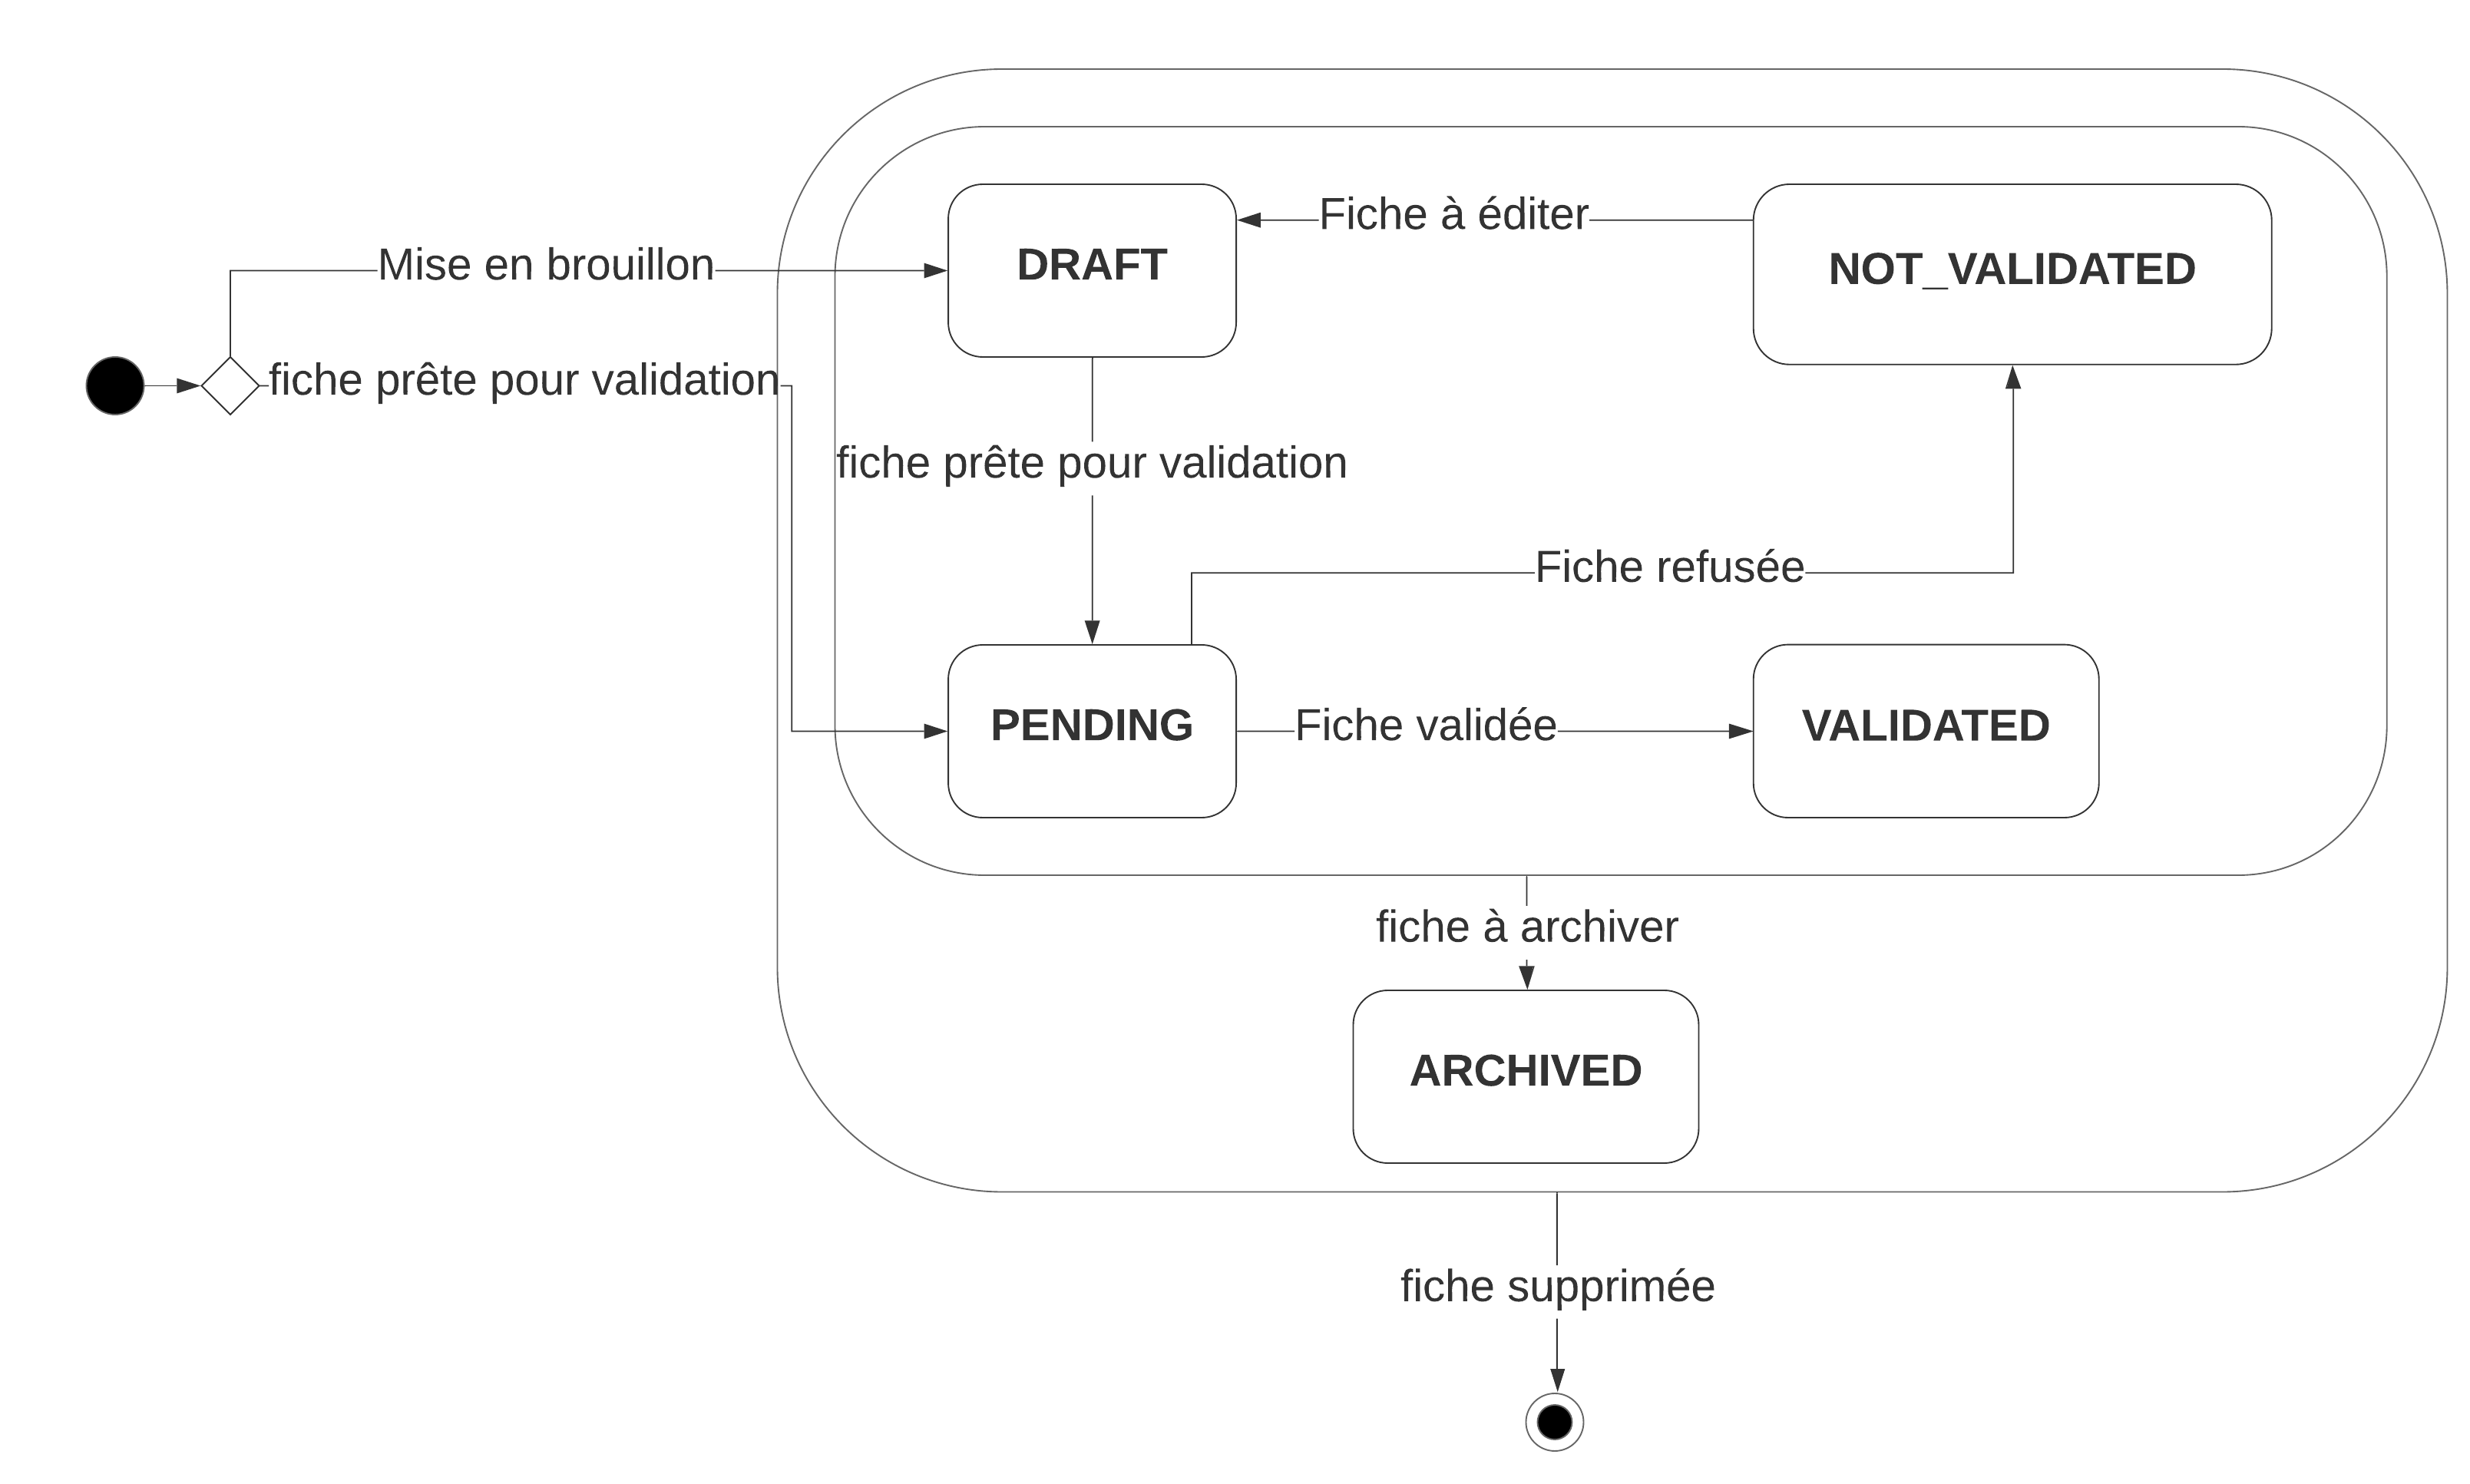
\includegraphics[width=\textwidth,height=\textheight,keepaspectratio]{images/StateFiches.png}
    \centering
    \caption{Diagramme UML à états pour l'état d'une fiche}
    \label{pic:stateDiagramForFiches}
\end{figure}

\subsection*{État d'un mot clé}

Une des questions annexes au sujet des fiches est la gestion des mots clés. En effet, les mots clés étant des éléments indispensables d'une fiche de qualité pour une meilleur référencement, il convient d'établir une stratégie précise pour exploiter au mieux ceux-ci. \\

Durant notre analyse, nous avons pu constater deux écoles de pensée bien distinctes (comparable à ce qui existe en économie) : 
\begin{itemize}
    \item laissez-faire : Il s'agit de donner une liberté totale en matière de marquage (en utilisant aussi bien des mots clés existants que non). Bien que cette approche a le mérite de faire émerger de nouveaux mots clés par les contributions d'utilisateurs, cela restreint les possibilités de modération.
    \item l'interventionnisme : Il s'agit de restreindre le choix en matière de marquage (exclusivement des mots clés existants). Bien que cette approche rend la modération facile, cela restreint les possibilités de s'adapter à une réalité changeante.
\end{itemize}

Nous avons remarqué qu'aucune de ces deux possibilités ne se distinguait suffisamment de l'autre pour répondre de manière optimale à la problématique.
C'est pourquoi nous avons fait le choix d'une 3e voie, qui se situe donc entre ces 2 manières de penser. Tout comme les fiches, il s'agit d'associer un état à chaque mot clé pour distinguer sa situation propre. Le diagramme UML à états ci-dessous représente ces états et les principales transitions entre états (pour ne pas surcharger celui-ci) :

% width=\textwidth,height=\textheight,keepaspectratio
\begin{figure}[H]
    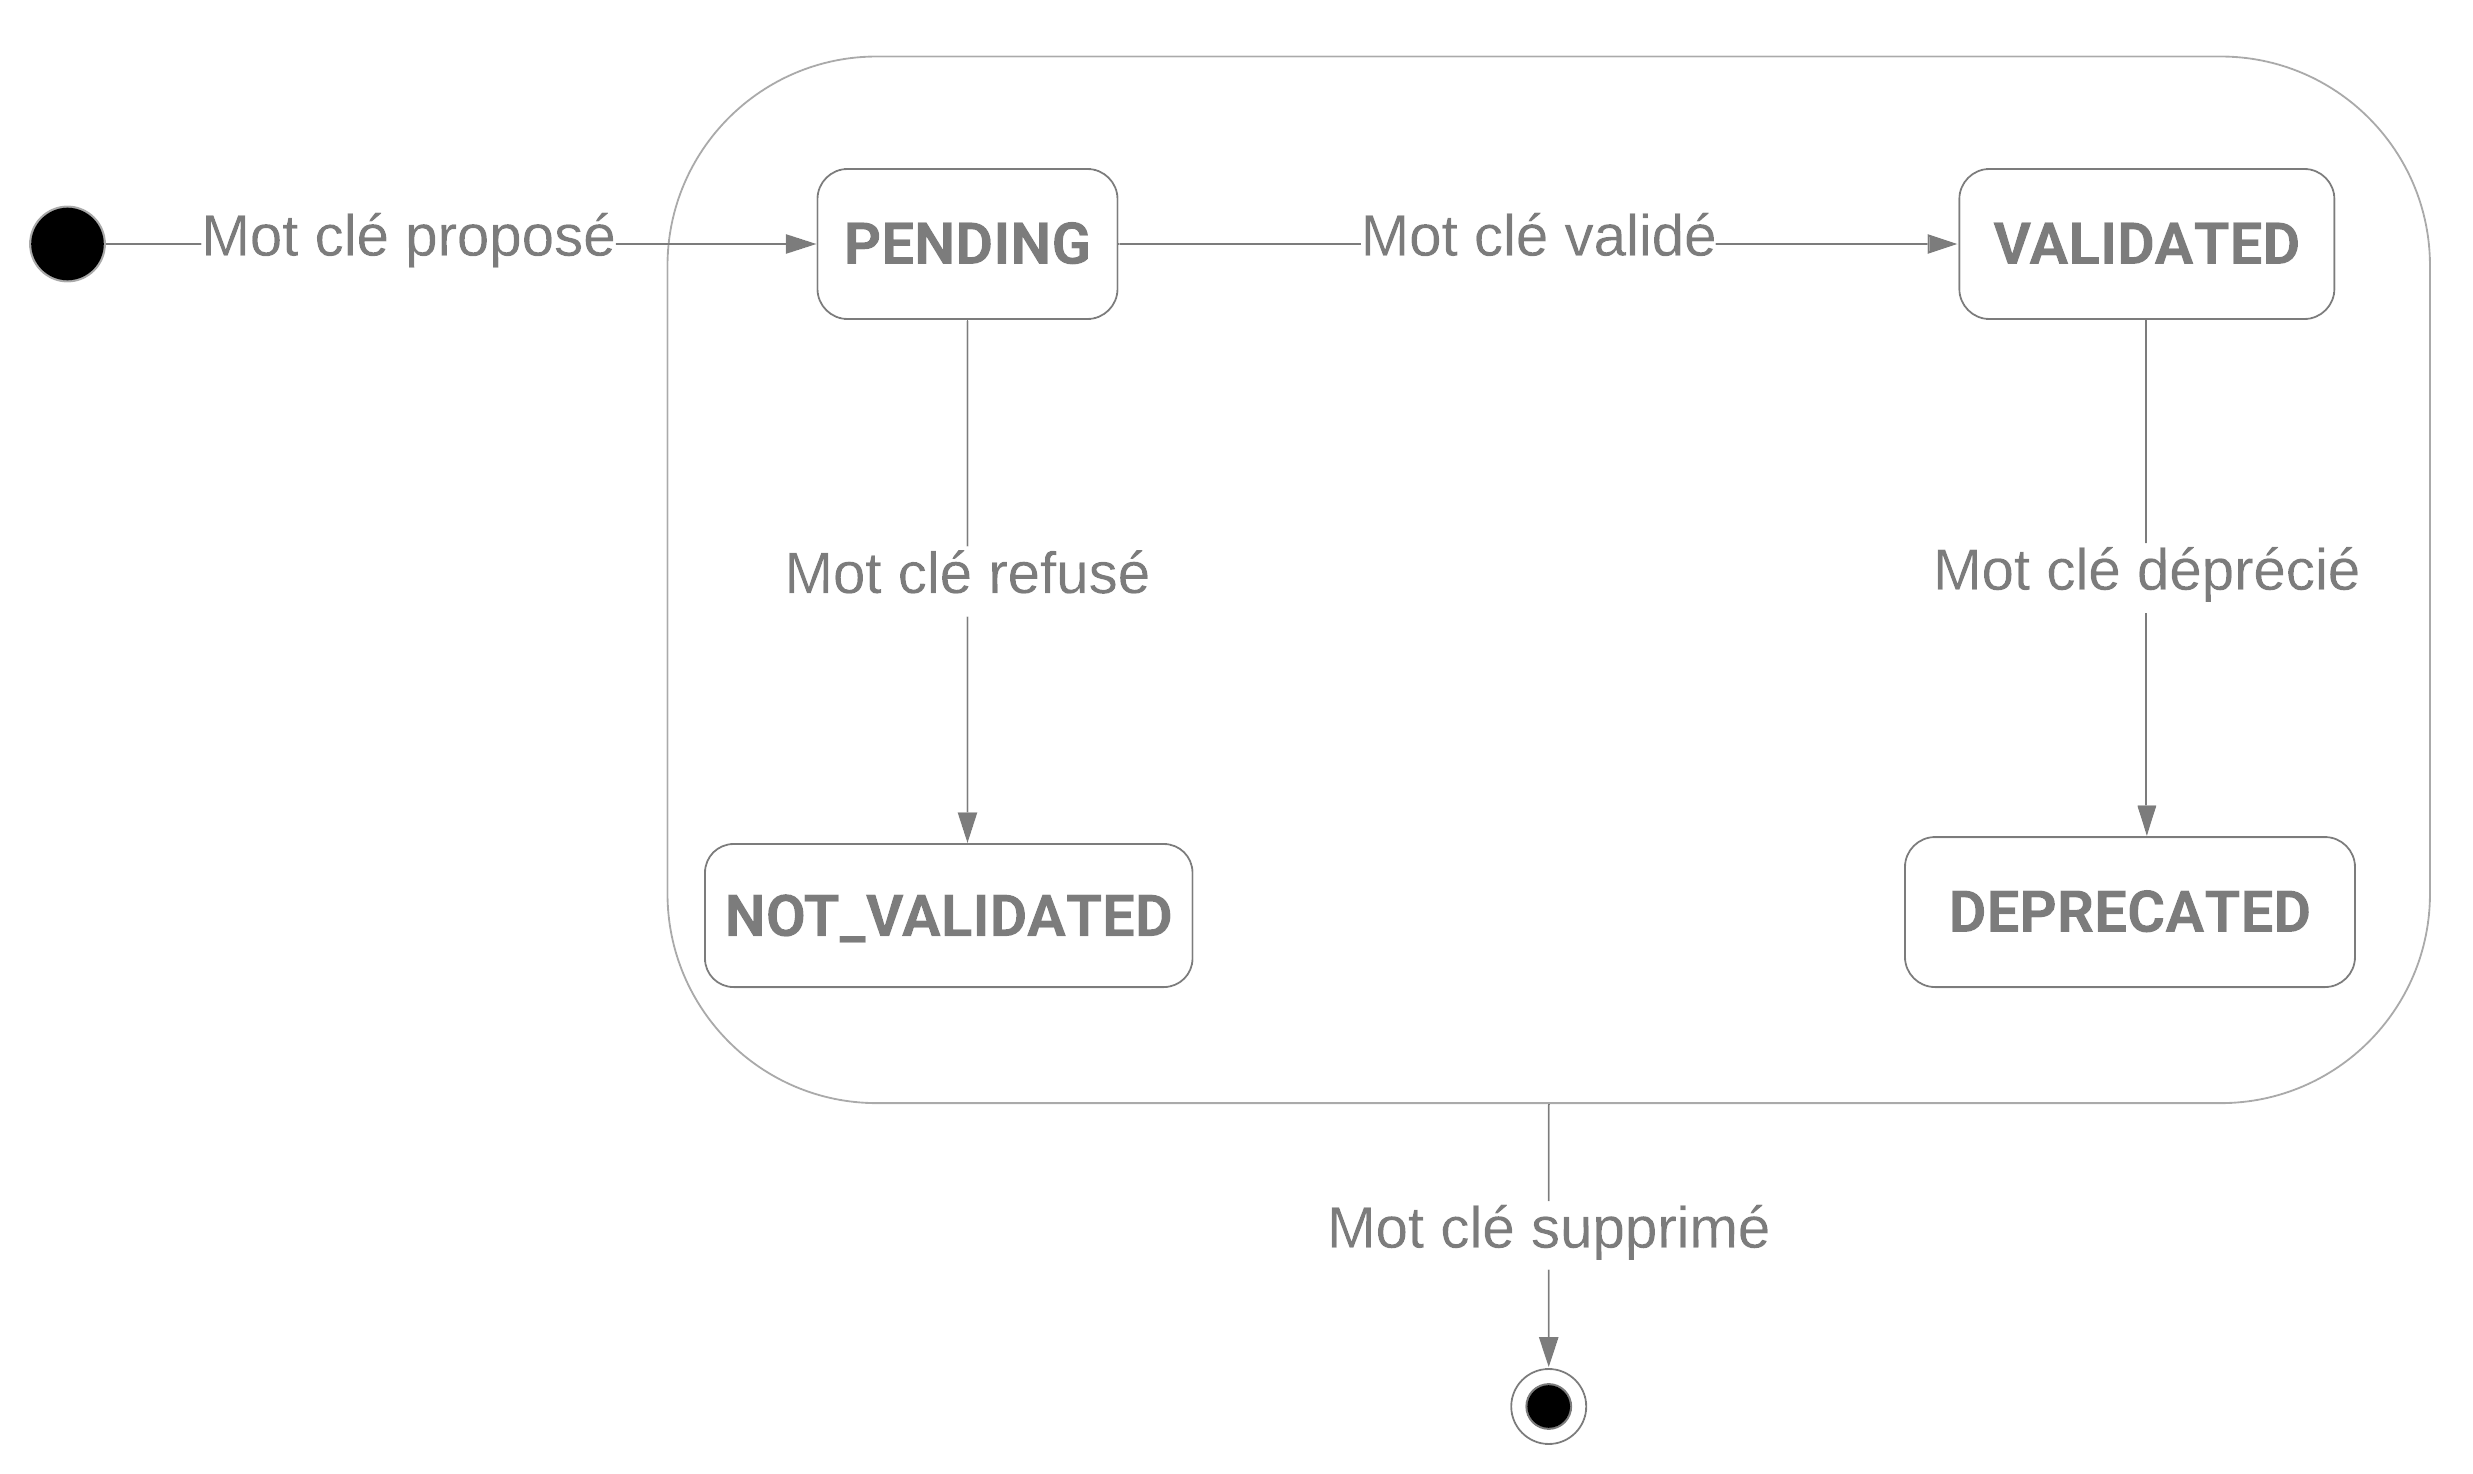
\includegraphics[width=\textwidth,height=\textheight,keepaspectratio]{images/StateTags.png}
    \centering
    \caption{Diagramme UML à états pour l'état d'un mot clé}
    \label{pic:stateDiagramForTags}
\end{figure}

\subsection*{Maintenabilité aisée des données}

Lors de notre analyse, un besoin particulièrement criant s'est présenté à nous : sans être informaticien ou connaître les technologies réalisant le stockage de données, il faut disposer d'un moyen de lire/modifier ces données avec aisance. \\

Cela implique dès lors de proposer des opérations pour manipuler les différentes ressources de notre application ( fiches, mots clés, catégories de mots clés, etc... ). Pour compléter la panoplie, nous avons conçu un moyen d'importer / exporter les fiches, notamment pour répondre aux besoins d'archivage.

\pagebreak


\section{Analyse non-fonctionnelle}
% On explique ici ( design, ergonomie )
% Donner les critères d'ergonomie
% Pas forcément des tonnes de page : à priori 3-4 max devraient suffire

\section {Contraintes}
% Expliquer les contraintes :
%    - Maintenabilité / Extensibilité  du code
%    - Gestion simple du système ( quand Mens disait que les admins ne devaient pas avoir à toucher à la DB pour faire x ou y truc )
%    - Interface orienté vers l'UX ( une jolie instruction UI VS UX
%    - etc...